\documentclass[parskip=full]{scrartcl}
\usepackage[T1]{fontenc}    % avoid garbled Unicode text in pdf
\usepackage[utf8]{inputenc} % use utf8 file encoding for TeX sources
\usepackage[german]{babel}  % german hyphenation, quotes, etc
\usepackage{hyperref}       % detailed hyperlink/pdf configuration
\hypersetup{                % ‘texdoc hyperref‘ for options
pdftitle={PSE: Entwicklung eines relationalen Debuggers - Implementierungsdokument},%
,%
}
\usepackage{graphicx}       % provides commands for including figures
\usepackage{csquotes}       % provides \enquote{} macro for "quotes"
\usepackage[nonumberlist]{glossaries}     % provides glossary commands
\usepackage{enumitem}
\usepackage{xcolor}
\usepackage{verbatimbox}
\usepackage{lscape}
\newcommand\frage[1]{\textcolor{red}{#1}}


\font\myfont=cmr12 at 16pt

\title{
	\vspace{2cm}
	\myfont 
	Praxis der Softwareentwicklung:\\ 
	Entwicklung eines relationalen Debuggers\\
}
\subtitle{
	\vspace{1cm}
	\myfont
	Implementierungsdokument
}
\author{
	\vspace{1cm} \\
	Benedikt Wagner\\
	\texttt{udpto@student.kit.edu}
	\and \vspace{1cm} \\ Chiara Staudenmaier\\
	\texttt{uzhtd@student.kit.edu}
	\and Etienne Brunner\\
	\texttt{urmlp@student.kit.edu}
	\and Joana Plewnia\\
	\texttt{uhfpm@student.kit.edu} 
	\and Pascal Zwick\\
	\texttt{uyqpk@student.kit.edu}
	\and Ulla Scheler\\
	\texttt{ujuhe@student.kit.edu}
	\vspace{1cm}
	\and Betreuer: Mihai Herda, Michael Kirsten
	\vspace{4cm}
}


\begin{document}
\clearpage
\maketitle
\pagenumbering{gobble}
\newpage

\tableofcontents
\newpage
\pagenumbering{arabic}

\section{Einleitung}
Dieses Dokument beschreibt die Ergebnisse der Implementierungsphase (\textit{08.01.-02.02.2018}) im Rahmen des Moduls Praxis der Softwareentwicklung (PSE) am Lehrstuhl \enquote{Anwendungsorientierte formale Verifikation - Prof. Dr. Beckert} am Karlsruher Institut für Technologie (KIT).\\
Hierbei handelt es sich um die Implementierung des Produkts \textit{DIbugger}, welches im Pflichtenheft definiert und während der Entwurfsphase entworfen wurde.

Das eigentliche Produkt dieser Phase ist über folgendes GitHub-Repository verfügbar: \href{https://github.com/JoanaP1997/PSE/tree/dev/Iplementierung}{https://github.com/JoanaP1997/PSE/tree/dev/Iplementierung} \\
Die abgegebene Version wurde mit \textit{release\_v1.0} getaggt.

\begin{figure}[!h]
\centering

\includegraphics[width=0.8\textwidth]{../Plichtenheft/logo_nongi.png}
\caption{Produktlogo}
\end{figure}

\section{Zeitablauf}
Um eine reibungslose Implementierung zu ermöglichen, muss ein gut durchdachter Zeitablauf existieren.
Dieser wurde folgendermaßen umgesetzt:\\
Begonnen wurde mit dem \textit{FileHandler} und dem \textit{UserInterface}. Diese konnten unabhängig voneinander implementiert werden.
Aus Zeitgründen verschob sich der Start der \textit{Control} Implementierung um wenige Tage.
Die Unterpakete der \textit{DebugLogic} wurden in planmäßiger Reihenfolge begonnen. Dabei wurde die \textit{DebugControl} nun parallel zum \textit{Interpreter} entwickelt.
Weiter gab es hier eine Änderung der Verantwortlichkeit: Ulla implementierte mit an dem Interpreterpaket, während Pascal den Debugger übernahm.
%folgend ein Bescheuerter Satz
Aus Interessen- und Vorwissensgründen wurde dies so abgesprochen und umgesetzt.
%Aufgrund des Vergessens von simplen Getter / Setter Methoden während des Entwurfs des Pakets \textit{FileHandler.Facade} hat sich die angedachte Entwicklungszeit stark vergrößert, da immer wieder kleine Änderungen vorgenommen werden mussten.%
Die Implementierung des \textit{Interpreters} war aufwändig, wie im Entwurf erarbeitet, allerdings stellte sich die Implementierung der Benutzeroberfläche als noch zeitintensiver heraus, was vor allem an der unintuitiven Bedienung der Bibliothek \textit{java.swing} lag. Diese gemeinschaftliche Fehleinschätzung wirkte sich auf auf die Erfüllung der funktionalen Anforderungen aus, wie im nächsten Abschnitt erklärt wird.
Das folgende Gantt-Diagramm zeigt den Zeitverlauf in graphischer Form auf.
\begin{figure}[!h]
\centering
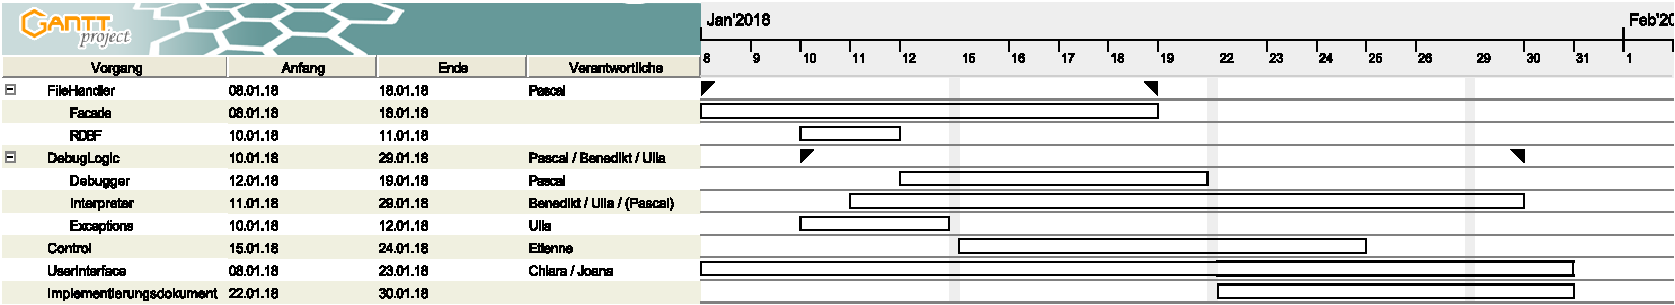
\includegraphics[width=1.0\textwidth]{ganntDiagramm_neu_2_crop.pdf}
\caption{Gantt-Diagramm des Zeitverlaufes}
\end{figure}

\section{Umsetzung der funktionalen Anforderungen}
Grundsätzlich ist zu sagen, dass der DIBugger die Funktion, für die er entworfen wurde, komplett erfüllt: Es ist möglich, mehrere Programme gleichzeitig zu debuggen und auf relationale Eigenschaften zu untersuchen.
Aus den im vorigen Abschnitt genannten Gründen, wurde eine Triage der Anforderungen vorgenommen, die dem Nutzer trotzdem die größtmögliche Funktionalität bereitstellen soll.

\subsection{Musskriterien}
Die Musskriterien wurden alle bis auf eines erfüllt. Dabei handelt es sich um /FA200/: \textit{\enquote{Die Variablenreihenfolge im Variableninspektor ist manuell veränderbar.}} \\ Dies ist in der aktuellen Version nicht möglich - Variablen können allerdings ein- und ausgeblendet werden. Auf den ersten Blick ist fraglich, warum es sich bei diesem Kriterium überhaupt um ein Musskriterium handelt. Grund dafür war der Folgende: Die Übersichtlichkeit der Benutzeroberfläche wurde als sehr relevant eingestuft, und es sollte dem Benutzer deshalb ermöglicht werden, die Werte zweier Variablen aus verschiedenen Programmen so zu verschieben, dass er sie leicht vergleichen kann. Mit der aktuellen Implementierung wird dieses Ziel aber trotzdem erreicht: Der Benutzer kann die für den Vergleich irrelevanten Variablen einfach ausblenden, sodass das Ziel der Übersichtlichkeit erfüllt wird.

\subsection{Sollkriterien}
Die Sollkriterien wurden alle bis auf eines erfüllt. Dabei handelt es sich um /FA230/: \textit{\enquote{Der Benutzer kann Variablen auswählen, von welchen jeder angenommene Wert gespeichert wird.}} \\
Dies ist in der aktuellen Version nur auf der Ebene der Benutzeroberfläche nicht möglich. Der Entwurf und die Implementierung des Interpreters unterstützen diese Funktionalität, da ein Trace alle Zustände einer Variablen enthält - und dies auch im Fall von Rekursion oder Schleifenaufrufen. Für eine Umsetzung auf der Benutzeroberfläche müsste noch ein weiteres Pop-Up und ein Menüeintrag hinzugefügt werden, worauf aus Gründen des Projektumfangs und der Zeit verzichtet wurde. Ist der Benutzer an allen Werten einer Variable interessiert, kann er diese Schritt (\enquote{Step}) für Schritt (\enquote{Step}) trotzdem einsehen. Hat der Benutzer eine konkrete Fragestellung bezüglich des Wertes einer Variablen, kann er diese über die Watch-Expressions und Bedingte Breakpoints überprüfen und die Fragestellung sogar mit Hilfe einer Bereichsbindung konkretisieren.

\subsection{Kannkriterien}
Das Kannkriterium /FA310/ wurde zuerst umgesetzt: \textit{\enquote{Der Benutzer kann Rückschritte in den Programmen durchführen.}} Dieses ist das wichtigste unter den Kannkriterien, da es eine Funktionalität bietet, die nicht anders erfüllt werden kann. \\
Nicht umgesetzt wurden:
\begin{itemize}
\item[/FA290/] \textit{\enquote{Die Datei des zu debuggenden Programms kann in eines der jeweiligen Textfelder hineingezogen werden.}} \\
Diese Funktionalität ist redundant zu /FA160/, /FA170/ und /FA180/, die bereits die Möglichkeiten bieten, Text direkt oder als Drag-and-Drop, per Copy-Paste oder als Textdatei einzubinden.
\item[/FA291/] \textit{\enquote{Die Textfelder für die jeweiligen Programme verfügen über ein Syntax-Highlighting.}} \\
Möchte der Benutzer ein Syntax-Highlighting haben, ist es ein Leichtes, den Programmtext erst in einem Editor zu verfassen und dann über die vielen verschiedenen Möglichkeiten der Texteinbindung im DIbugger einzufügen.
\item[/FA320/] \textit{\enquote{Die an Zeilen im Programm gebundenen Breakpoints verschieben sich mit dem Programm, wenn dieses im Editiermodus geändert wird.}}  \\
Problematisch hierbei ist, dass das JPanel, indem sich der Programmtext befindet, Änderungen am Text nicht direkt erfasst. Um Breakpoints korrekt zu verschieben, müsste die Benutzeroberfläche somit nach jedem einzelnen Klick in einem Programmfenster, den gesamten Inhalt Zeile für Zeile parsen und ihn mit dem vorigen Text zu vergleichen. Auf Grund dieser unattraktiven Lösung wurde das Kriterium zurückgestellt.

\end{itemize}


\section{Umsetzung der nichtfunktionalen-Anforderungen}

Die Einteilung der nichtfunktionalen Anforderungen in Unterkapitel orientiert sich an der Anordnung im Pflichtenheft. Wenn eine Anforderung bezüglich ihrer Relevanz klassifiziert wurde, ist dies auch aufgeführt.			
			 
		\subsection{Produktleistungen}
		%Zeitverhalten, Genauigkeit, Fehlertoleranz
		\begin{itemize}
		\item[/PL10/] Zeitverhalten: \\ Wie im Pflichtenheft gefordert, ist das Hinzufügen von Eingabevariablen, Watch-Expressions, Schrittgrößen und Breakpoints ohne spürbare Verzögerung möglich. Selbiges gilt für das Ausführen von Schritten, Step-Over und Step-Out. Erreicht wurde dies dadurch, dass der \textit{Trace} beim Starten des Debugmodus zunächst vollständig erzeugt wird. Operationen davor und danach können dadurch sehr schnell durchgeführt werden. Das Starten des Debugmodus selbst gelingt im Rahmen der bereits getesteten Programme deutlich unter 5 Sekunden. Genauere Zusicherungen können hier erst nach der Testphase gemacht werden.
%		Das Produkt ermöglicht das Hinzufügen von Eingabevariablen, Watch-Expressions, Schrittgröße und Breakpoints ohne spürbare Verzögerung. Das Ausführen von Schritten, Step-Over und Step-Out, sowie das Erreichen des nächsten Breakpoints, ist ebenfalls ohne spürbare Verzögerung möglich. \\
		%Den Debugmodus zu starten dauert unter 5 Sekunden. 

		\item[/PL20/] Genauigkeit: \\
		Da die Sprache alle primitiven Datentypen von Java unterstützt und diese im Produkt durch äquivalente Java Typen, laufend auf einer JVM (Java Virtual Machine), implementiert wurden, ergeben sich dieselben Genauigkeiten auch bei Ausführung von Programmen der Sprache WLang. Die im Pflichtenheft dokumentierten Anforderungen wurden damit umgesetzt.

		\item[/PL30/] Fehlertoleranz: \\
		Die Fehlertoleranz, im Pflichtenheft als relevant eingestuft, wurde durch verschiedene Maßnahmen umgesetzt: Erstens, werden bei fehlenden Eingabewerten für Startvariablen diese automatisch generiert. Zweitens, wird die Semantik aller Eingaben (das heißt von Eingabevariablen, Programmtexten, Watch-Expressions und Bedingten Breakpoints) beim Start des Debugmodus direkt vom \textit{Antlr}-Parser kontrolliert. Dabei auftretende Fehler werden durch Pop-Ups über die Benutzeroberfläche zurückgemeldet.
%		Durch automatische Warnung bei kritischen Eingaben (A10, A20) und Überprüfung der Semantik, ergibt sich eine hohe Fehlertoleranz bezüglich Benutzereingaben.
%		Durch die automatische Generierung von fehlenden Benutzerangaben für Eingabewerte (FA215), wird der Start des Debugmodus aus dem Editiermodus bei korrektem Programmtext zu jeder Zeit ermöglicht.
%		Über andere Arten von Fehlern wird der Benutzer mittels Pop-Ups informiert.
		\end{itemize}
		
		Unter dem Punkt \enquote{Qualitätsanforderungen an das System} wurde im Pflichtenheft außerdem genannt:
		\begin{itemize}
		\item Richtigkeit: \\
		Die Richtigkeit wurde im Pflichtenheft als sehr relevant eingestuft. Die Implementierung hat dies so weit wie möglich berücksichtigt. Die tatsächliche Umsetzung kann allerdings erst während der Qualitätssicherung sichergestellt werden.
		\item Installierbarkeit: \\
Der DIbugger wird in einer zip-Datei abgeliefert, die eine ausführbare jar-Datei enthält.		
		
		\end{itemize}
		
		\subsection{Weitere nichtfunktionale Anforderungen}
		%Benutzbarkeit, Wartbarkeit, Erweiterbarkeit, Gesetze/Normen/Sicherheit/Urheberrecht, Robustheit
		\begin{itemize}
		\item[/NA10/]Erweiterbarkeit: \\
		Die Erweiterbarkeit wurde durch klare Pakettrennung, Fassadenklassen als Eintrittstellen in die Pakete und die Definition von Interfaces und abstrakten Klassen (z.B. die abstrakte Klasse \textit{InputValueSuggestion} im Paket \textit{debuglogic.debugger}) sichergestellt und erleichtert.
		\item[/NA20/]Wartbarkeit: \\
		Zunächst fördert die eben dargelegte Umsetzung der Erweiterbarkeit natürlich auch die Wartbarkeit des Produktes. Während der Implementierung wurde außerdem auf eine vollständige und verständliche Dokumentierung Wert gelegt. Die Einarbeitungszeit in den Programmcode wird so verringert.
		\item[/NA30/]Urheberrecht: \\
		Die geplante Open Source Lizenz \href{https://www.gnu.org/licenses/gpl-3.0.de.html}{GNU GPL 3 (GNU General Public License)} wurde im GitHub-Repository als Lizenz eingetragen.
		
		\item[/NA40/] Sicherheit: \\
		Wie bereits im Pflichtenheft festgelegt, gilt: Da das Produkt keine Netzwerkverbindung nutzt, verbleiben die vom Benutzer eingegebenen Daten zumindest im Zuständigkeitsbereichs des Programmes ausschließlich auf dem Rechner des Benutzers.
		\item[/NA50/]Benutzerfreundlichkeit: \\
		Auf Benutzerfreundlichkeit wurde großen Wert gelegt. Eine genauere Aufschlüsselung der Maßnahmen nach Verständlichkeit, Übersichtlichkeit und Erlernbarkeit ist im nächsten Absatz zu finden.
%		Durch das Hilfemenü werden dem Benutzer die wichtigsten Funktionen und deren Anwendung des Produkts erklärt. Erklärungen zu Bestandteilen der Benutzeroberfläche sind durch Tooltips abgedeckt. \\
%		Durch die strikte Trennung der verschiedenen und Gruppierung der zusammengehörigen Elemente der Benutzeroberfläche ergibt sich ein übersichtliches Erscheinungsbild. 
		\end{itemize}
		
				Unter dem Punkt \enquote{Qualitätsanforderungen an die Benutzeroberfläche} wurden im Pflichtenheft außerdem genannt:
				\begin{itemize}
				\item Verständlichkeit \\ 
				Die Verständlichkeit der Benutzeroberfläche wurde im Pflichtenheft als relevant eingestuft. Dazu wurde auf eine klare Bezeichnung aller Buttons geachtet und Konventionen aus handelsüblichen Debuggern, wie zum Beispiel in Eclipse, wurden weitestgehend übernommen. 
				\item Übersichtlichkeit \\
				Die Übersichtlichkeit der Benutzeroberfläche wurd im Pflichtenheft als sehr relvant eingestuft. Dem wurde Rechnung getragen, indem die Benutzeroberfläche möglichst simpel gehalten und klar strukturiert ist. Funktionen, die seltener genutzt werden, wie die Auswahl einer Sprache, wurden in die Menüleiste eingebunden. Die Entscheidung, ob ein Button mit Text oder mit einer Zeichnung beschriftet wird, wurde auf individueller Basis getroffen, um Übersichtlichkeit und Verständlichkeit zu fördern.
				\item Erlernbarkeit \\
				Die Erlernbarkeit der Benutzeroberfläche wurde im Pflichtenheft als relevant eingestuft. Verständlichkeit und Übersichtlichkeit tragen dazu natürlich bei - vor allem wurde aber eine Dokumentation erstellt, die über den Hilfe-Menüeintrag verfügbar ist und eine Übersicht über das Programm gibt, sowie häufige Fehlerquellen im Umgang mit dem Produkt, insbesondere der benutzten Sprache WLang, adressiert. Endgültige Aussagen zur Erlernbarkeit können allerdings erst nach der Testphase getroffen werden, wenn mehrere, entwicklungsfremde Testpersonen der Zielgruppe (das heißt Individuen, die bereits Erfahrung mit üblichen Debuggern und Programmiersprachen haben) das Produkt benutzt haben. Die Dokumentation wird dann um ihre Fragen und Anmerkungen erweitert.
				\item Modifizierbarkeit \\
				Die Modifizierbarkeit, im Pflichtenheft bezogen auf das Hinzufügen zusätzlicher Funktionalität bei Veränderungen am Code des DIbuggers, wurde als sehr relevant eingestuft. Um eine optimale Modifizierbarkeit zu leisten, hätte man eine neue Bibliothek zur Erstellung von Benutzeroberflächen entwerfen und implementieren müssen. Dies war im Rahmen dieses Projektes jedoch nicht vorgesehen. Innerhalb der Einschränkungen von \textit{java.swing} wurden mittels klarer Dokumentation und der Verwendung von \textit{JPanels} allerdings trotzdem die Bedingungen für eine möglichst hohe Modifizierbarkeit geschaffen. Soll zusätzliche Funktionalität hinzugefügt werden, kann dies einfach über ein neues \textit{JPanel} geschehen.
				
				\end{itemize}
		
\section{Umsetzung von Entwurfsentscheidungen}
%\subsection{Model-View-Control}
%\subsection{Das Observerpattern}
%z.B. Gui-Facade
%\newpage
\subsection{Singleton}
%%z.B. Command Panel
Durch die Nutzung von Rekursion und des Singletons der Klasse RDBFParser, siehe Abbildung \ref{loadRDBF}, kann das Einlesen einer RDBF (Relational DIbugger Format) Datei in einer kurzen Methoden geschehen.
Über \textit{evaluateLineType(String line)} wird der Typ einer Zeile herausgefunden. Je nachdem, von welchem Typ diese Zeile dann ist, werden über das Singleton der Klasse RDBFParser unterschiedliche Methoden aufgerufen, um eine Zuweisung oder einen Block zu erstellen und in der Dateistruktur einzuordnen. Dies ist durch das Singleton einfach zu lösen.
\begin{figure}[!h]
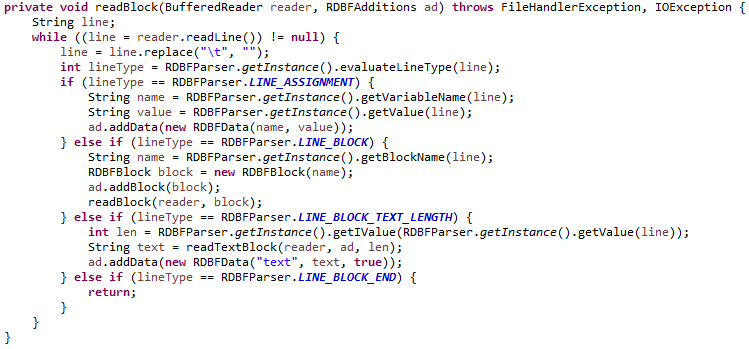
\includegraphics[width=1.0\textwidth]{document_data/loadRDBFFile.png}
\caption{Nutzung des Singletons der Klasse RDBFParser}
\label{loadRDBF}
\end{figure}

%\subsection{Fassade}
%z.B. Control-Facade

\newpage
\subsection{Strategie}
%z.B. FileWriter
\begin{figure}[!h]
\centering
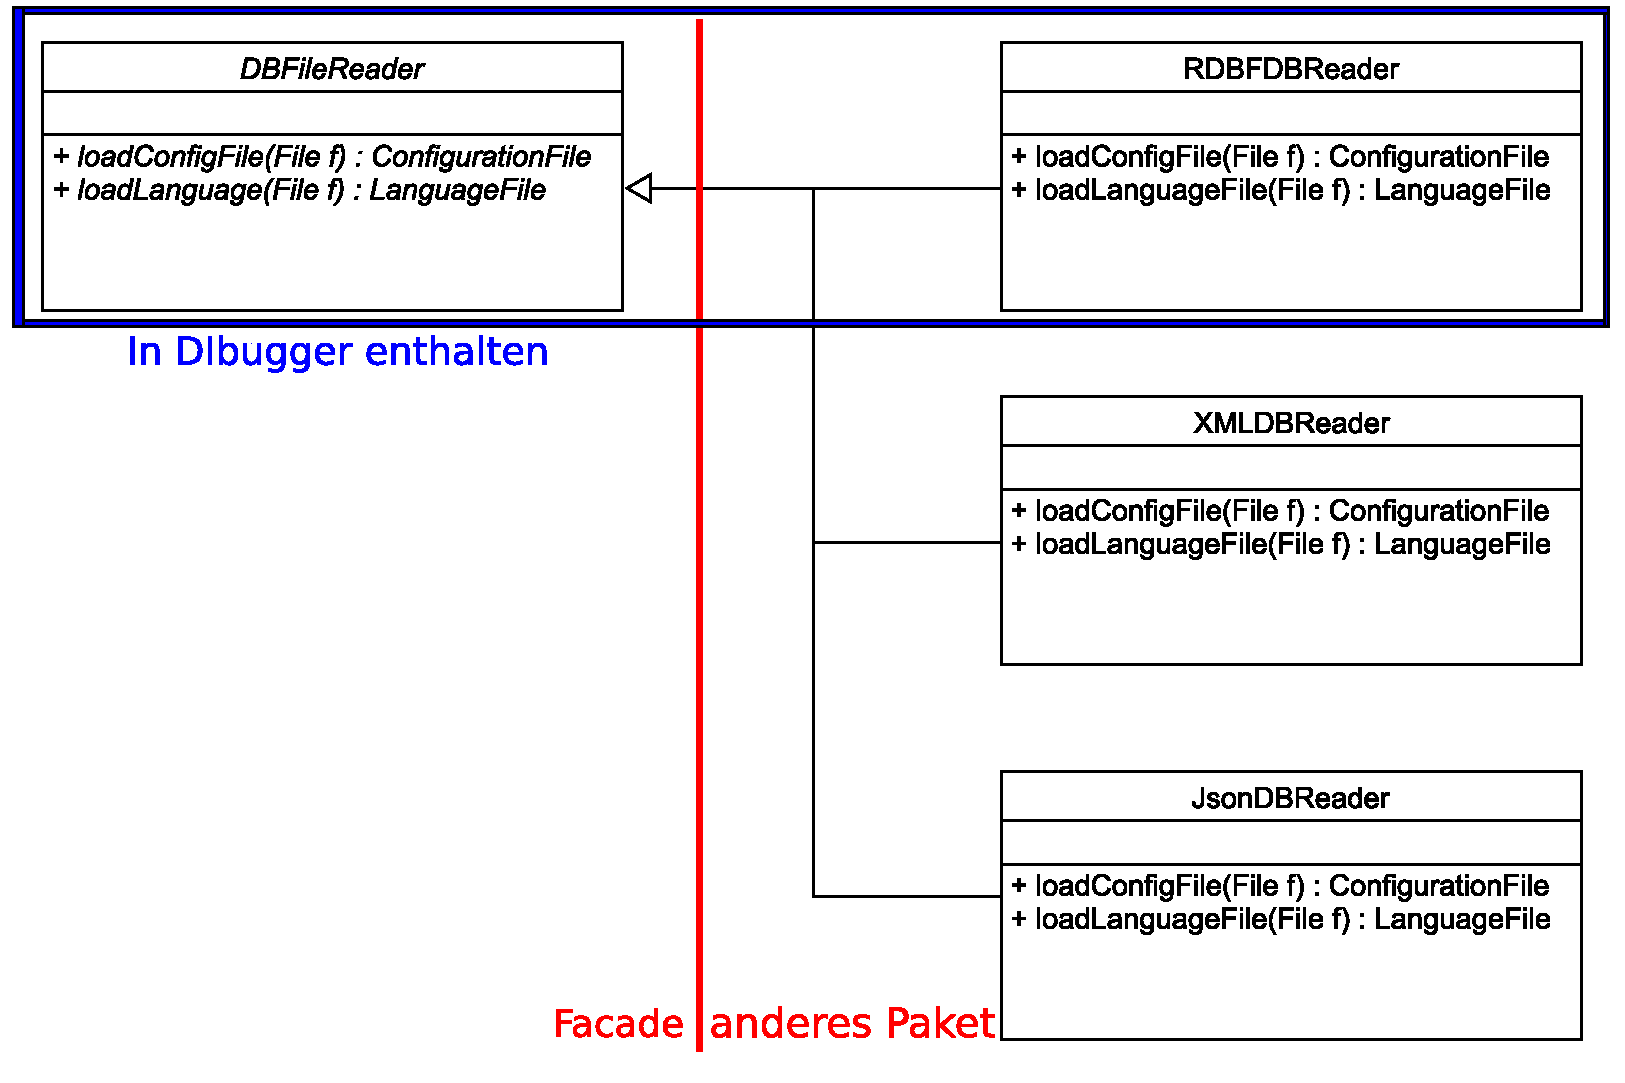
\includegraphics[width=0.8\textwidth]{document_data/Strategy_uml_d.pdf}
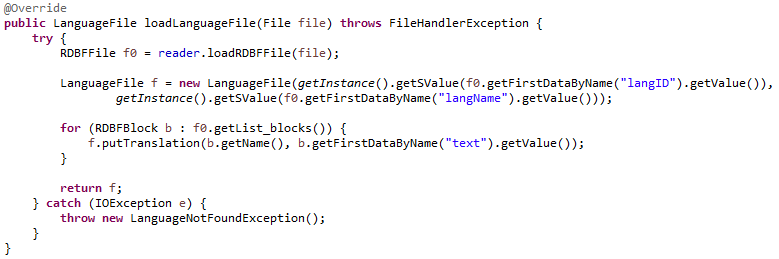
\includegraphics[width=1.0\textwidth]{document_data/loadLangFile.png}
\caption{Strategiemuster des DBFileReaders im Paket FileHandler}
\label{fig:strategy_fh}
\end{figure}
Wie in Abbildung \ref{fig:strategy_fh} aufgezeigt, steht der DBFileReader (der Klassenname steht für \enquote{DebuggerFileReader}) für den \enquote{Kopf} des Strategiemusters.
Dieser kann als abstrakte Klasse nicht erzeugt werden und stellt zwei abstrakte Methoden ohne Implementierung zur Verfügung.
Diese müssen bei der Vererbung durch eine Unterklasse, z.B. \textit{RDBFDBFileReader} (der Klassenname steht für enquote{RelationalDebuggerFormatDebuggerFileReader}), \textit{XMLDBFileReader}, \textit{JsonDBFileReader} usw., überschrieben und vollständig Implementiert werden.
Dadurch können unter Vorraussetzung einer korrekten Implementierung der beiden Methoden weitere Dateiformate hinzugefügt werden.
Dies gilt ebenso für die Klassen \textit{DBFileWriter, PropertiesFileReader} und \textit{PropertiesFileWriter}. Sie sind ähnlich aufgebaut zu der hier gezeigten Klasse.

\subsection{Die Visitor im Interpreter} Der Entwurf sah im Paket \textit{Interpreter} zwei Klassen vor, die das Visitor Pattern umsetzen. Die beiden Klassen \textit{CommandGenerationVisitor} und \textit{TermGenerationVisitor} sind Unterklassen der von Antlr generierten Klasse \textit{WlangBaseVisitor<T>}, wobei der Generic hier angibt, welchen Datentyp die visit-Methoden zurückgeben. Wie es der Name andeutet, ist dies zum einen die Klasse \textit{Command} und zum anderen die Klasse \textit{Term}. 
Da Terme sowohl während der Traceerzeugung (genauere Erklärung dazu ist im Entwurfsdokument Kapitel 8.10 zu finden) als auch innerhalb von Watch-Expressions und bedingten Breakpoints vorkommen, kam das Problem auf, dass der \textit{TermGenerationVisitor} zunächst sowohl vom \textit{TermsBaseVisitor} (für die im Entwurfsdokument Anhang 12.2 definierte Syntax der Watch-Expressions) als auch vom \textit{WlangBaseVisitor} (für die in Entwurfsdokument 12.1 definierte Wlang-Syntax) erben musste. In Java ist bekanntlich keine Mehrfachvererbung möglich. Zur Lösung des Problems wurden die Grammatiken zusammengefügt und entsprechend beim Verwenden eine andere Startregel angegeben. 
\subsection{Nutzung der von Antlr generierten Klassen}
In Abbildung \ref{createTerm} ist die Nutzung der von Antlr generierten Klassen im Rahmen einer Watch-Expression zu sehen. Wenn diese Klassen benutzt werden, geschieht das immer wie in den Zeilen 65-68. Im einzelnen Fall muss dann nur die richtige Startregel der Grammatik ausgewählt werden, hier zum Beispiel \textit{webppterm()} (\enquote{webppterm} steht für \enquote{watch-expression-bedingter-Preakpoint-Term)}. \\
Im abgebildeten Code ist in \texttt{this.specifier} der String gespeichert worden, der die Watch-Expression spezifiziert. Die Klassen \textit{WlangLexer} und \textit{WlangParser} erzeugen dann einen Ableitungsbaum, den \textit{ParseTree}. Über diesen werden die oben angesprochenen Visitor geschickt.
\begin{figure}[!h]
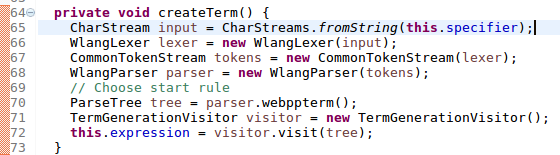
\includegraphics[width=0.7\textwidth]{document_data/createTerm.png}
\caption{Aufrufen der von Antlr erzeugten Klassen}
\label{createTerm}
\end{figure}

\subsection{Umsetzung der Commands}
Die Klassen \textit{Command} und ihre Unterklassen wurden wie im Entwurfsdokument spezifiziert als Kompositum implementiert. Dabei haben zusammengesetzte Subklassen wie der \textit{WhileCommand} immer eine \textit{addChild(Command child)}-Methode. Kritisch an den Commands ist vor allem die Umsetzung ihrer \textit{run()}-Methode. Diese ist einer der wichtigsten Teile der Umsetzung des Interpreterpaketes. Sobald sich hier ein Fehler einschleicht, werden die Programmausführungen fehlerhaft. Deshalb wird es wichtig sein, in der Qualitätssicherungsphase diesen Teil besonders ausgiebig zu testen. Bereits in der Implementierung wurden die Commands durch Unittests auf ihr Verhalten überprüft. 
Als einfaches Beispiel betrachten wir in Abbildung \ref{runWhile} die \textit{run()}-Methode der Klasse \textit{WhileCommand}. Hier wird der Nutzen des Kompositum Musters ersichtlich.
Zunächst wird in jedem Command der aktuelle \textit{Scope} vom hauptverantwortlichen \textit{GenerationController} \texttt{this.controller} geholt. In einfachen Befehlen (z.B. \textit{Assignment}) wird dieser einfach nur manipuliert. Hier müssen wir die Bedingung der While-Schleife auswerten, um zu sehen, ob diese sich überhaupt zu einem Boolean auswertet (Zeile 38-39). Dann prüfen wir je einmal die Bedingung und führen alle Kinder mit \textit{run()} aus. Das passiert solange die Bedingung sich zu wahr auswertet (Zeile 45-49). Da wir immer im gleichen Scope bleiben, muss die oben angesprochene Typprüfung nur einmal erfolgen.
\begin{figure}[!h]
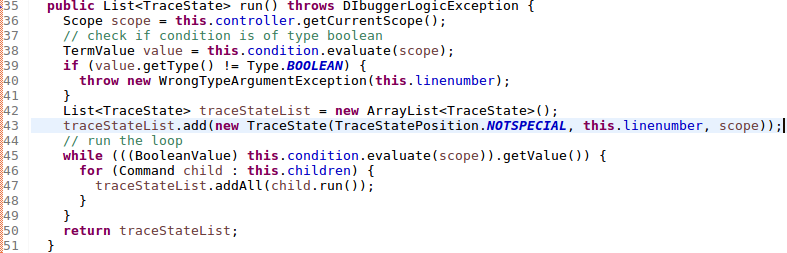
\includegraphics[width=1.0\textwidth]{document_data/runWhile.png}
\caption{run()-Methode der Klasse \textit{WhileCommand}}
\label{runWhile}
\end{figure}
\section{Änderungen zum Entwurf}

\subsection{UserInterface}
\paragraph{ExpressionChangePopUp}
Der Entwurf wurde aus Gründen der Übersichtlichkeit um die Klasse \textit{ExpressionChangePopUp}, die von \textit{DIbuggerPopUp} erbt, ergänzt. Ein \textit{ExpressionChangePopUp} dient dabei dem Löschen und Ändern der Bereichsbindung einer WatchExpression oder eines bedingten Breakpoints.
\paragraph{ArrayValuePopUp}
Die im Entwurf spezifizierte Klasse \textit{ArrayValuePopUp}, eine Unterklasse von \textit{DIbuggerPopUp}, wurde in der Implementierung aus Gründen der Benutzerfreundlichkeit verworfen. Ursprünglich sollte sie das Eintragen der Werte eines Arrays über ein PopUp erleichtern. Mit Hilfe eines Scrollbalkens im Variableninspektor ist es allerdings möglich, Werte für Arrays auf dieselbe Art und Weise wie Werte für andere Datentypen einzugeben.
\paragraph{ProgramPanel}
ProgramPanels werden nun nicht mehr über Integers identifiziert, sondern über Strings (A-Z). So ist innerhalb des Modells gewährleistet, dass auch nach Löschung eines einzelnen ProgramPanels die zu den Programmen gehörigen Variablen in Watch-Expressions und bedingten Breakpoints korrekt angezeigt werden.
\subsection{Control}
\paragraph{ExceptionHandler}
Damit Fehlermeldungen in der richtigen Sprache ausgegeben werden, ist der \textit{ExceptionHandler} nun ein Beobachter (im Beobachter-Entwurfsmuster) und beobachtet \textit{FileHandlerInteractor}, um über Änderungen der Benutzersprache informiert zu werden.
\paragraph{FileHandlerInteractor}
Es besteht nun eine Assoziation zwischen \textit{FileHandlerInteractor} und \textit{DebugLogicFacade}, da so \textit{ControlFacade} weniger Funktionalität besitzt, die \textit{FileHandlerInteractor} zuzuordnen ist.
Weiter ist diese Klasse Subjekt im Beobachter-Entwurfsmuster, sodass Objekte anderer Klassen benachrichtigt werden können, falls \textit{FileHandlerInteractor} beispielsweise andere Konfigurationen verwaltet als zuvor.
\paragraph{TextInputBuffer}
Die Klasse \textit{TextInputBuffer} wurde hinzugefügt, um die Parameter der Eingabewerte, Porgrammtexte und -identifikatoren, welche in \textit{Control} zwischenzuspeichern sind, zu kapseln.
Eine Instanz dieser Klasse ermöglicht es genau ein solches \enquote{Tripel} (Eingabewerte, ...) zu speichern und als \textit{ProgramInput}-Objekt wieder abzurufen.
\subsection{FileHandler}
%+ FileHandlerFacade: savePropertiesFile()
\paragraph{Exceptions Paket}
Das Exceptions-Paket sah eine Oberklasse \textit{FileHandlerException} als Interface vor.
Alle Unterklassen, welche diese Schnittstelle implementieren, sollten von der Klasse \textit{java.lang.Exceptions} erben. Da aber Schnittstellen in Java nicht geworfen werden können, wurde die Schnittstelle \textit{FileHandlerException} zu einer abstrakten Klasse mit Erbschaft von \textit{java.lang.Exception}.
\subsection{DebugLogic}
\subsubsection{Debugger}
%+ DebugLogicFacade: extends Observable statt Subject \\
%* DebugLogicFacade: notifyObservers(Object arg); suggestStepSize void statt String \\
%+ DebugControl: setStepSize(programID, stepSize); reset();
\paragraph{Subject}
Im Entwurf wurde die Klasse \textit{Subject} spezifiziert. Sie ist Kontrollpunkt des Beobachtermusters zwischen GUI und DebugLogic. Da eine äquivalente Klasse aus Java, namentlich \textit{Observable}, existiert, wurde die Klasse \textit{Subject} nicht implementiert.
\textit{Observable} bietet die gleichen Methoden an wie die im DIbugger definierte Klasse.
\paragraph{DebugLogicFacade}
Diese Klasse erbt nun von der Java Klasse \textit{Observable} anstatt von \textit{Subject}.
Aus den oben genannten Gründen kann somit auch auf die Implementierung der in \textit{Subject} enthaltenen Methoden verzichtet werden.

\subsubsection{Interpreter}
\paragraph{TraceIterator}
Ursprünglich sollte der \textit{TraceIterator} mit Hilfe einer gesonderten Klasse gleichen Namens umgesetzt werden. In der Implementierung wird er nun mittels eines Java-ListIterators über die \textit{TraceState}-Liste innerhalb der Klasse \textit{Trace} verwirklicht. Dieser bietet dieselben Funktionalitäten, kann also in zwei Richtungen iterieren. Um einen Iterator über den Trace zu erhalten, wird weiterhin die Methode \textit{iterator()} der Klasse \textit{Trace} aufgerufen. Diese Entwurfsänderung stellt somit lediglich eine Vereinfachung dar.
\paragraph{TermValue}
Die Klasse \textit{TermValue}, die ursprünglich als Interface implementiert werden sollte, ist nun eine abstrakte Klasse. So kann die Methode \textit{getType()} einmal an zentraler Stelle für alle Unterklassen definiert werden und Code-Duplikate werden vermieden.
\paragraph{TraceState}
In der Klasse \textit{TraceState} wurde das Attribut String programId ergänzt. Dies ist nötig, damit WatchExpressions - die nur TraceStates und keine Traces kennen - wissen, zu welchem Programm welcher TraceState gehört. Dies hat auch eine Änderung in den Klassen \textit{Trace} und \textit{GenerationController} zu Folge. Die Klasse \textit{Trace} übernimmt die Aufgabe, die eben beschriebene \textit{programId} in alle \textit{TraceStates} eines \textit{Traces} einzutragen, und nimmt dazu in ihrem Konstruktor einen weiteren Parameter entgegen. Da der \textit{Trace} diese Information vom  \textit{GenerationController} bekommt, wird auch in letzterem der Konstruktor erweitert.
\subparagraph{Zusätzliche Klassen}
Um das entgegennehmen von Rückgabewerten bei Funktionsaufrufen in einem Wlang-Programm zu ermöglichen, wurde der neue Befehl \textit{CallingAssignment} eingeführt. Durch die Erweiterbarkeit des Entwurfsmusters Kompositum konnte diese Klasse einfach als neue Unterklasse von \textit{Command} eingebaut werden. Die übrigen Klassen konnten so die neue Klasse ohne Änderung nutzen.\\
Ebenso wurde die Klasse \textit{TermList} als neue Unterklasse der Klasse \textit{Term} ins Termkompositum eingebaut. Diese war notwendig, um Starteingaben des Nutzers der Form \texttt{a = \{1,3,1,5\}} zu ermöglichen. Auch hier konnte der erweiterbare Entwurf ausgenutzt werden, sodass diese Neueinführung keine weiteren Änderungen veranlasste.
Zudem wurden die zusätzlichen Exception Klassen \textit{SyntaxException, WatchExpressionSyntaxException} und \textit{ConditionalBreakpointSyntaxException} eingefügt. Diese sorgen für spezifiziertere Fehlermeldungen an den Nutzer.
\subsubsection{Antlr}
\paragraph{ActuallyHelpfulException und ActuallyHelpfulErrorListener}
Ursprünglich sollte das gesamte Antlr-Paket autogeneriert werden. Allerdings mussten zur Behandlung von Exceptions zwei Klassen hinzugefügt werden, da Antlr standardmäßig alle Fehlermeldungen auf das Terminal schreibt, statt sie zu werfen.

 

\end{document}
